\documentclass{urticle}

\begin{document}

\begin{center}
{\LARGE \textbf{Исследование коннектом и когнетом}}

{\Large Мокров Никита}

{\large Московский Физико-Технический Институт}

{\large Факультет Радиотехники и Кибернетики}

{\large mokrov@frtk.ru}
\end{center}

\section*{Введение}
\subsection*{Постановка задачи}
Термин «коннектом» предложен в 2005 году независимо двумя исследователями Олафом Спорнсом и Патриком Хэгмэнном по аналогии с «геномом» (полное описание всех генов) и «протеомом» (полное описание строения и функций всех белков). Сегодня под «коннектомом» понимают полное описание связей в нервной системе того или иного организма.

Как известно, главной задачей нейронаук является понимание того, как из работы материальных и доступных изучению приборами элементов нервной системы получается неуловимая работа психики. Создание сетевых моделей формальных элементов мозга (когнитома) — всего лишь один из этапов. Наш соотечественник Константин Анохин вводит новый термин «ког» — элемент психического опыта, связанный с работой какого-то участка нейронной сети. Из множества связанных друг с другом когов строится когнитом — сеть психики, внутренний мир животного или человека, которому принадлежит данная нейронная сеть.

С точки зрения математики процесса, мы можем представить человеческий мозг в виде взвешенного графа взаимодействия отедльных его участков. Этот факт дает широкие возможности для большого спектра задач. 

Одна из таких - задача машинного обучения. Как по коннектому и когнетому человека, определить определенную болезнь человека на ранней стадии.

\subsection*{Методы решения и новые подходы}
На данный момент эта задача решается широким кругом лиц из всех стран мира. Исследование в данном отчете основывается на работе по повышению классификации путем сочетания различных нормировок\cite{article1}\cite{article2}.

В данной работе приведены слудующие методы нормализации:
\begin{itemize}
	\item Оригинальная нормализация
	\item Бинарная нормализация
	\item Геометрическая нормализация
	\item Топологическая нормализация			
\end{itemize}

Данный подход смог учесть различные характеристики графа и помог улучшить результат.

\section*{Альтернативный подход}
В данной статье использовались данные людей здоровых и больных аутизмом (UCLA Multimodal Connectivity Database), которые содержат порядка 100 матриц смежности размера (264, 264) для графов, которые и представляют когнетом пациента.

В связи с этим возникает проблема большой размерности, вследсвтии чего, большого числа признаков. В данной работе была проверена теория о том, что исходные данные сильно зашумлены. Во-первых, это следует из того, что каждая нервная клетка обновляет силу связи между смежными нейронными, и поэтому мы строим модель для опрделенного момента времени и состояния человека. Во-вторых, данная теория появилась вследствии того, что исходный графы, а значит и матрицы, были получены путем срванения послойных участков мозга вручную.

Для решения этой проблемы, воспользуемся спектральным разложением (Или что тоже самое для симметричной матрицы - сингулярное разложение). 
$$ A = V \Lambda {V}^{-1} $$
После чего, будет использовать вместо матрицы $A$, матрицу $A'$
$$ A' = V \Lambda $$
Дальше, убирая k столбцов матрицы V, соответсвующие наименьшим собственным знаениям, и соответсвуенно в матрице $\Lambda$ сами собственные значения, мы получаем из матрицы размера (N, N), матрицу размера (N, N-k). И эту новую матрицу будем использовать как целевую переменную.

\section*{Результаты}
Так для чистых данных, которые никак не нормализуюутся и не перевзвешиваются, значение по метрике ROC AUC для 100 валидаций выглядит следующим образом.

\begin{figure}[H]
	\centering{
	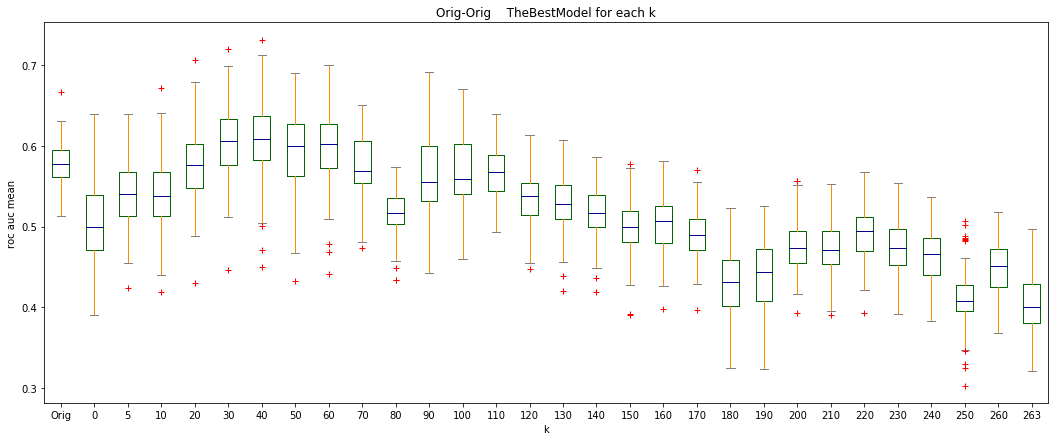
\includegraphics[width=160mm]{1.png}
	}
	\caption{Boxplot для оригинальной матрицы в зависимости от $k$}
	\label{f1}
\end{figure}

Чаще всего так получается, что лучшее решение заключается в объединении двух или более других. Перед тем как понижать размерность матрицы $A$, можно по-разному ee нормализовать.
Если вопспользоваться бинарной нормировкой, то результат смотрится гараздо лучше.
\begin{figure}[H]
	\noindent\centering{
	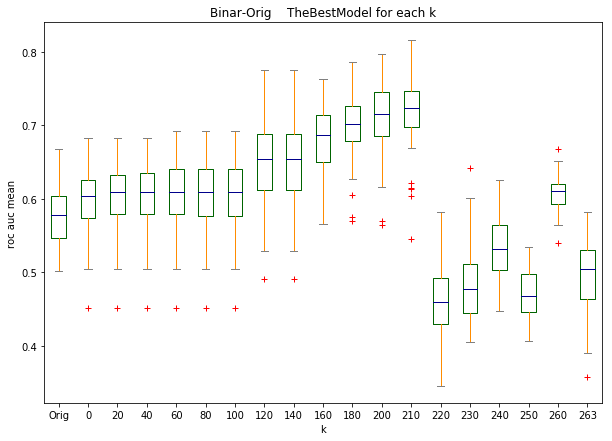
\includegraphics[width=120mm]{2.png}
	}
	\caption{Boxplot для бинарной матрицы в зависимости от $k$}
	\label{f}
\end{figure}

Данный метод был опробован на дргуих данныx (APOE-4), которые содержат пары (матрица размером (68, 68) и метка класса). Проведем тот же алогритм на бинарной нормировке и получим такие значения для 100 валидаций.

\begin{figure}[H]
	\noindent\centering{
	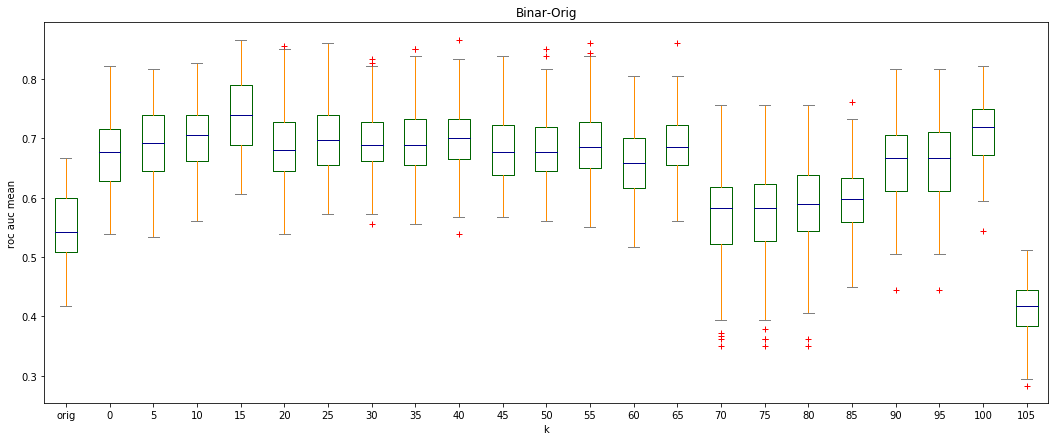
\includegraphics[width=160mm]{3.png}
	}
	\caption{Boxplot для бинарной матрицы в зависимости от $k$}
	\label{f3}
\end{figure}


\section*{Заключение}
Как можно заметить, используюя только более информативные признаки матрицы (собственные вектора, умноженные на собственные значения), результат может улучишься для правильной первоначальной нормировки данных.

В заключении хотелось бы отметить, что по ходу исследования возникали новые вопросы, на которые пока нет четких ответов.

\subsection*{Используемая литература}
\begin{thebibliography}{2}
\bibitem{article1} Boosting Connectome Classification via Combination of Geometric and Topological Normalizations by Dmitry Petrov, Yulia Dodonova, Leonid Zhukov and Mikhail Belyaev
\bibitem{article2} Machine Learning Application to Human Brain Network Studies: A Kernel Approach by Anvar Kurmukov, Yulia Dodonova and Leonid Zhukov 
\end{thebibliography}

\end{document}
